\section{Study}
To investigate the efficacy of action suggestions, we conducted a between-subjects experiment in which participants edited their own photos in Photoshop. In the experimental condition, subjects had access to Discovery\-Space; in the control condition they did not. We hypothesized that participants exposed to the suggestions in Discovery\-Space would find the editing process easier, feel more creative, and become more confident using Photoshop. 

\subsection{Method}
To sign up, participants completed a brief initial survey about their Photoshop experience. Participants were then scheduled for a 30-minute session and assigned to one of two conditions: participants in the Discovery\-Space condition used Photoshop with the Discovery\-Space panel open, and participants in the Control condition used Photoshop with a blank panel that instructed them to save their photo when finished (\autoref{fig:discoveryspace_exp_interface}). The study held constant the length of the session (30 minutes), the number of photos edited (two), the questions participants answered when opening and closing a photo, and the availability of a web browser (yes).

\begin{figure}[b!]
\centering
  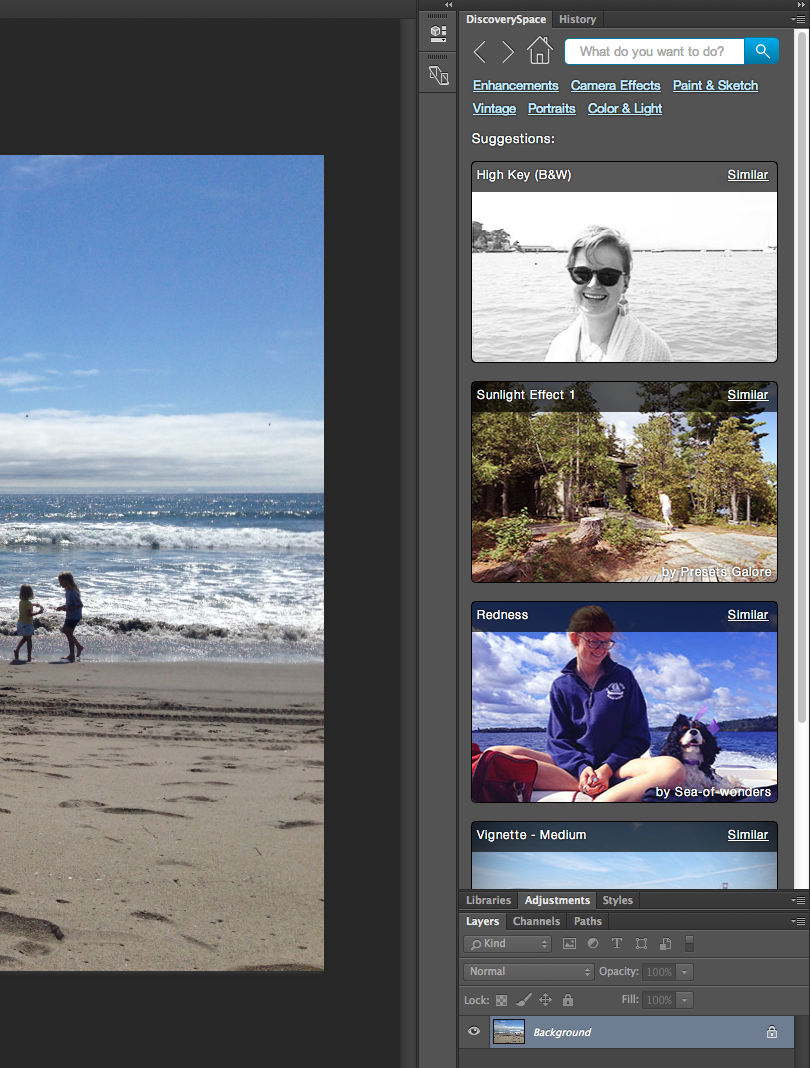
\includegraphics[width=0.4\textwidth]{discoveryspace/figures/experiment-DS.png}
  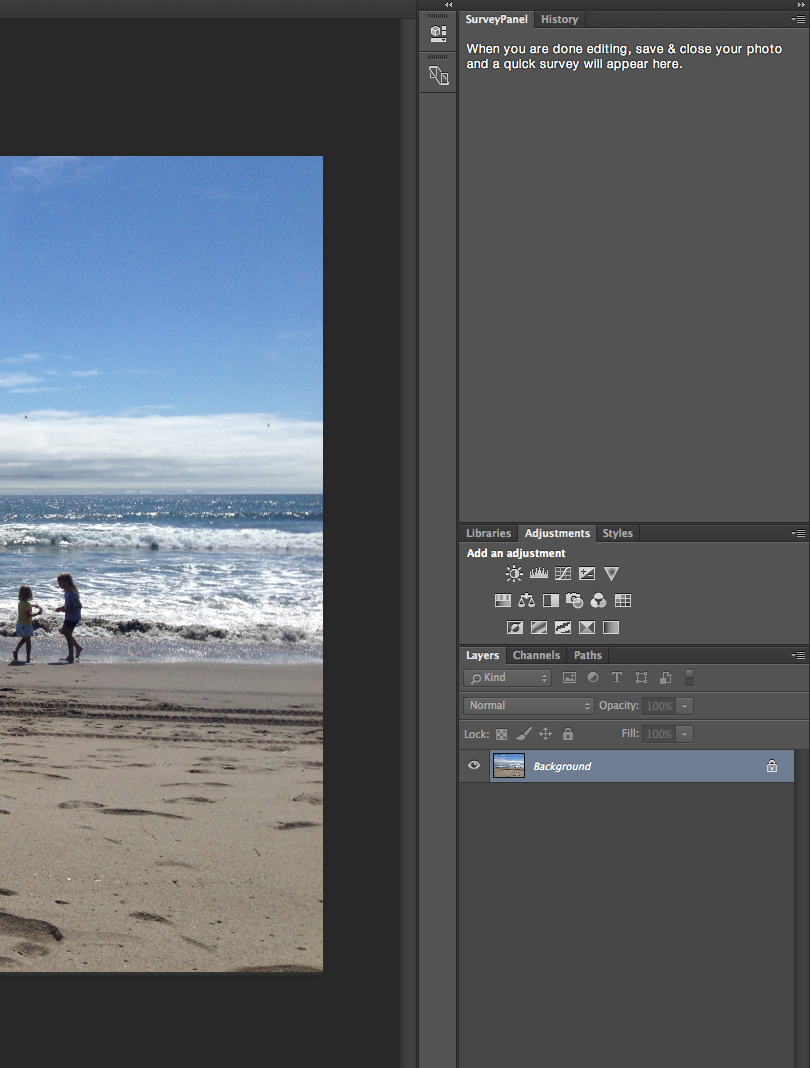
\includegraphics[width=0.4\textwidth]{discoveryspace/figures/experiment-C.png}
  \caption{Photoshop as it appeared in the DiscoverySpace condition (left) and Control condition (right).}~\label{fig:discoveryspace_exp_interface}
\end{figure}

Each session comprised the following steps: consent form, background questions, edit first photo, edit second photo, short interview, and final online survey. The background questions allowed participants to elaborate on their initial survey responses regarding their prior experience with Photoshop and photo editing. Participants were instructed to bring one photo containing at least one person, and one photo without people, to ensure some consistency across participants' photos. The editing order of the two photos was randomly assigned with balancing in each condition. We chose to allow participants to bring their own photos, rather than provide sample photos, so that participants would be more likely to come up with their own goals for their photos, and would be motivated to do a good job. 

\begin{figure}[b!]
\centering
  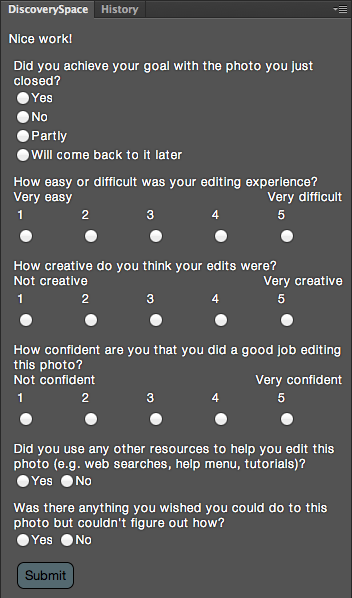
\includegraphics[width=0.5\textwidth]{discoveryspace/figures/close_questions.png}
  \caption{Questions answered by participants after editing each photo. The measure for ``How confident are you that you did a good job editing this photo?'' is referred to as ``confidence about performance'' in the Results.}~\label{fig:discoveryspace_close}
\end{figure}

In both conditions, upon opening a photo, the study panel prompted the user to describe their goal for the photo and select its image features. The panel also prompted the user to answer a few questions about their editing experience every time a photo was closed (\autoref{fig:discoveryspace_close}). The panel was in a prominent location and the participants were made aware of it by the experimenter. The task was open-ended: participants could define their goal however they wanted and were simply instructed to work until they were satisfied (or until time ran out).  We used an open-ended task as opposed to a more directed one because participants would be more likely to perform as they would in a real-world setting when working on personally meaningful tasks. In the Discovery\-Space condition, participants were given a quick overview of the Discovery\-Space interface and were shown what each button in the panel did, so that time would not be wasted figuring out how to use the interface. The History panel was located behind Discovery\-Space, and was only visible when clicked on. Participants in the Discovery\-Space condition were shown the History panel only if they asked explicitly how to go back in time by more than one action. 

In both conditions, a web browser was open on the Google home page just behind Photoshop; participants were told they could use it at any time. This was included to reflect the ready availability of web resources in creative workflows. A short interview and final survey took place in the last five minutes of the session. It comprised follow-up questions on the participant's overall editing experience and their perceived difficulties. 

\subsection{Participants}
28 students were recruited from four undergraduate classes at a Southern California university (one photography class, three design classes). None of these classes provided formal training in Photoshop, though many participants had experience with other photo editing software and/or basic photography principles. Stratified randomization was used to balance gender and Photoshop expertise across conditions. Expertise with Photoshop was measured as follows: in the initial survey, participants were asked to rate their skill level with Photoshop from 1 to 5, and their amount of experience with Photoshop from 1 to 5. The answers to these two questions were added together to produce a score between 2 and 10, and participants were grouped according to their score into Beginner (2-4), Intermediate (5-7) and Expert (8-10). See \autoref{table:ds_participants} for the distribution of participants' expertise and gender. 15 participants were assigned to the Discovery\-Space condition, and 13 to the Control condition (the uneven balance was due to the stratified randomization).

\begin{table}[t]
\centering
\caption{Participants' gender and Photoshop expertise.}~\label{table:ds_participants}
\begin{tabular}{l|lll}
 & Female & Male & \textbf{Total} \\ \hline
Beginner & 6 & 5 & \textbf{11} \\
Intermediate & 3 & 9 & \textbf{12} \\
Expert & 1 & 4 & \textbf{5} \\
\textbf{Total} & \textbf{10} & \textbf{18} & \textbf{28}
\end{tabular}
\end{table}

\subsection{Measures}
Both surveys asked participants to rate their Photoshop confidence by answering two questions: ``How confident are you with your ability to edit photos in Photoshop? (1-5)'' and ``How confident are you that you can achieve your goals in Photoshop? (1-5)''. We measured change in confidence as the difference between the sum of both responses (between 2 and 10) in the final survey and the initial survey. For each of the three Likert-scale questions answered after every photo (\autoref{fig:discoveryspace_close}), we added the responses from both photos to obtain one score between 2 and 10 for each participant ($N = 28$). For the questions with yes/no answers, we considered each photo separately ($N = 56$ as each participant edited two photos). We also recorded the number of Photoshop tools used (not including those from Discovery\-Space) and all clicks and pages loaded in Discovery\-Space.

\subsection{Results}
For the numerical measures, we used analysis of variance to analyze Condition, Expertise, and their interaction. For yes/no measures, we used logistic regression with the same variables. 

\subsubsection{Participant goals}
As expected with such an open-ended task, there was a large variety of participant goals. The most frequent goals focused on color/brightness (\textit{e.g.}, ``correct exposure and color balance'' or ``experiment with color''), or a particular emotional effect (\textit{e.g.}, ``make it surreal looking'' or ``give a lonely, solemn feel''). As expected, participants more often (72\% of the time) used non-technical terms to describe their goals rather than photography-specific terms such as ``saturation'' and ``sharpness''. This was most prominent among Beginners and Intermediates.

\subsubsection{Quantitative results}
Beginner participants in particular were significantly more likely to lose confidence in the Control condition ($M = -2.0$) and gain confidence in the Discovery\-Space condition ($M = 0.5$), $t(22) = -2.16, p = 0.04$ (\autoref{fig:discoveryspace_confidence}). Across all Expertise levels, Discovery\-Space had only a marginal effect on participants' confidence: the confidence of Control participants decreased ($M = -0.77$) while the confidence of Discovery\-Space participants increased ($M = 0.27$), but this was not significant, $F(1, 22) = 2.97, p = 0.10$. No effect was found for Expertise. 

\begin{figure}[t!]
\centering
  \includegraphics[width=0.6\textwidth]{discoveryspace/figures/confidence-new.png}
  \caption{Confidence of Beginner Control participants decreased while confidence of Beginner Discovery\-Space participants increased. Error bars show 1 standard error from the mean. Note that due to small sample sizes in the sub-conditions, this is intended only as a descriptive illustration.}~\label{fig:discoveryspace_confidence}
\end{figure}

\begin{table}[t]
\centering
\caption{Summary of mean values for measures compared between conditions. Discovery\-Space participants had marginally \textit{higher} confidence change (this effect was significant within the Beginner group), and stated they could not figure something out \textit{less often} than Control participants.}~\label{table:ds_results}
\begin{tabular}{l|l|l|l}
 & DiscoverySpace & Control & $p$ \\ \hline
\textbf{Total confidence change (-8 – 8)} & \textbf{0.27} & \textbf{-0.77} & \textbf{0.10} \\
\textbf{Couldn’t figure something out = yes} & \textbf{50\%} & \textbf{80\%} & \textbf{0.02} \\
Achieved goal = yes & 47\% & 31\% & 0.72 \\
Used web browser & 33\% & 54\% & 0.26 \\
Difficulty (2 – 10) & 5.3 & 6.0 & 0.37 \\
Creativity (2 – 10) & 4.5 & 4.1 & 0.86 \\
Confidence about performance (2 – 10) & 5.9 & 5.2 & 0.68 \\
\# Photoshop tools used & 15 & 20 & 0.38
\end{tabular}
\end{table}

Discovery\-Space participants were significantly less likely to state that there was something they couldn't figure out ($M = 50\%$) than Control participants ($M = 80\%$), $\chi^2(1) = 5.52, p = 0.02$. 

All measures compared between conditions are summarized in \autoref{table:ds_results}. Responses to many of the post-editing questions varied widely. Within the Beginner group, Discovery\-Space participants rated difficulty as marginally but not significantly lower ($M = 5.3$) than Control participants ($M = 6.8$), $t(22) = 1.62, p = 0.12$. 

Across both conditions, Experts rated difficulty significantly lower ($M = 4.4$) when compared against Intermediates ($M = 5.8$) and Beginners ($M = 6.0$) together, $t(22) = -2.14, p = 0.04$. Experts also used significantly more tools ($M = 26$) than Intermediates ($M = 16$) and Beginners ($M = 16$), $t(22) = 2.37, p = 0.03$. In the Discovery\-Space condition, 51\% of the actions used were radical and 49\% were refinement, which suggests both types of actions were useful.

Overall, there was a strong negative correlation between difficulty and confidence about performance, $r(28) = -.70, p < .0001$. Interestingly, there was also a strong positive correlation between creativity and confidence about performance, $r(28) = .67, p < .0001$.  This effect seems to hold most strongly for Beginners, as the correlation was weaker for Intermediates and Experts only, $r(17) = 0.48, p = 0.05$. Further exploration revealed that using the web was negatively correlated with achieving one's goal, $\chi^2(1) = 8.09, p = .005$, and positively correlated with having trouble figuring something out, $\chi^2(1) = 6.93, p = 0.01$.

Preliminary analyses found no effects for type of class (photography vs. design), so this was excluded from further analyses. Gender was confounded with Expertise (\autoref{table:ds_participants}) so Gender was also excluded from analyses; however within the Beginner group where Gender was roughly balanced, no Gender effects were found.

\subsubsection{Qualitative results}
Participants were asked at the end of the session if they had discovered any new effects or tools. All Discovery\-Space participants replied yes, most of them adding that Discovery\-Space had exposed them to effects they had not seen before. 9 of 13 Control participants also responded yes, that they had discovered a new tool, mainly by clicking around or from an online tutorial. Two added that while they had discovered a new tool, they were unsure how to use it.

Discovery\-Space participants were asked two additional questions about the kinds of tasks for which they might use Discovery\-Space, and about the capabilities they wish it had. The most popular response to the task question was ``for making quick and fun edits'', such as preparing a photo to post on social media or editing personal photos for fun, as opposed to aiming for professional-looking or detailed edits. The capabilities most participants wished Discovery\-Space had were more control over the result of an effect, such as sliders to dial it down or to adjust its parameters; and the ability to apply the effect to a selected part of the image only. Other requests included an explanation as to how the effect was achieved so that the user could easily repeat it and experiment with it, and better interaction with the document history. Though users could go back and forward through the applied operations using the History panel, it is separate from Discovery\-Space, and does not allow editing of the previous steps.

Discovery\-Space participants were also given the opportunity to share their general thoughts about the panel. Most stated either that they found it helpful, or that it had the potential to be helpful if some of the aforementioned improvements were made. Novice participants in particular seemed on the whole excited by Discovery\-Space as it meant they were able to achieve effects they otherwise would not have thought possible.
